\chapter{Grundlagen}
\label{chap:grundlagen}

\section{\acf{scm}}

\acl{scm}, auch \acs{scm} genannt, dient dazu Versionen von Softwarekomponenten zu verwalten und wird verwendet, um Änderungen an einem Quellcode \textit{Repository} zu verfolgen und die Historie aller Änderungen nachzuvollziehen. Das \textit{Repository} bezeichnet dabei den Speicherort von Softwarekomponenten. Grundsätzlich soll es allen Mitwirkenden eines Projekts helfen, Aktualisierungen an einer Codebasis zusammenzuführen. Oft wird \ac{scm} als Synonym für \ac{vcs} verwendet \citep{scm_atlassian}.

\section{\textit{Git-Workflow} und \textit{Pull Requests}}

Ein solches \ac{scm} ist \textit{Git}, welches Änderungen an einer Codebasis verwaltet und dokumentiert \citep{git}. Üblicherweise wird die Codebasis eines Projektes im \ac{scm} System auf dem \textit{master}-\textit{Branch} verwaltet. Vom \textit{master}-\textit{Branch} wird auf den \textit{developer}-\textit{Branch} abgezweigt, von dem aus die Entwicklung startet. Eine Änderung, z.\,B. in Form einer neuen Funktionalität wird dann beispielsweise auf einem \textit{feature}-\textit{Branch} entwickelt. Dieser entspringt dem \textit{developer}-\textit{Branch} und wird am Ende der Entwicklung wieder in den \textit{developer}-\textit{Branch} integriert. Basierend auf dem \textit{developer}-\textit{Branch} werden \textit{release}-\textit{Branches} erzeugt, auf denen \textit{Release}-Versionen auf Produktivumgebungen getestet und gegebenenfalls \textit{Bugs} behoben werden. Ist der \textit{Release} vollständig, so wird der \textit{release}-\textit{Branch} sowohl in den \textit{developer}- als auch den \textit{master}-\textit{Branch} integriert. Dieser Prozess dient der besseren Zusammenarbeit und Skalierung des Entwicklungsteams und wird als \textit{Git-Workflow} bezeichnet \citep{git_workflow_atlassian}. 

Das Zusammenführen der \textit{Branches} und der damit verbundene Arbeitsablauf wird allgemein als \textit{Pull Request} bezeichnet und wird immer von einem anderen Mitglied aus dem Team geprüft (\textit{Review}) und anschließend akzeptiert (\textit{Merge}) oder abgelehnt (\textit{Close}). Durch den \textit{Pull Request} signalisiert der Entwickler also die Fertigstellung seines Beitrags und bittet somit um die Prüfung der Änderung und das Zusammenführen in die Codebasis, fasst \citet{fowler_2021} zusammen. Je nach verwendetem \ac{scm} System, wird der \textit{Pull Request} teilweise auch als \textit{Merge Request} bezeichnet \citep{fowler_2021}.

Das Konzept der \textit{Branches}, der \textit{Git-Workflow} und der darin enthaltene Prozess des Pull Requests wird in \autoref{fig:pr-flow} beschrieben.

\begin{figure}[ht!]
\centering
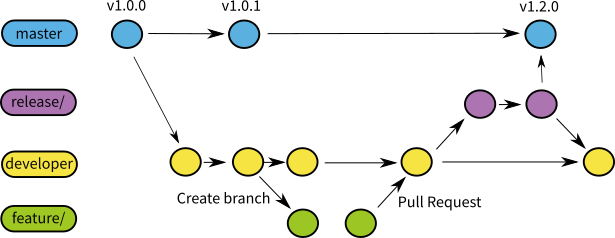
\includegraphics[width=\textwidth]{source/images/pr-flow}
\caption[Visualisierung des \textit{Git-Workflows}.]{Visualisierung des \textit{Git-Workflows}, Quelle: Eigene Darstellung nach \citealt{contribution_workflow}.}
\label{fig:pr-flow}
\end{figure}


\section{\acf{ci}}

Der Begriff \acl{ci}, auch \ac{ci} genannt, entstammt der Software Entwicklung und beschreibt dabei einen Prozess der permanenten Integration. Wie \citet{jenkins-guide} beschreibt, war es in den frühen Anfängen der Softwareentwicklung üblich, dass alle Änderungen der beteiligten Team Mitglieder zu einem Zeitpunkt, der sogenannten Integrationsphase, in der Codebasis vereint wurden und daraus ein \textit{Release} erzeugt wurde. 
Diese Phase ging in der Regel mit harter Arbeit und monatelangem Lösen von Konflikten einher, da diese nur schwer vorherzusehen sind. Noch schwieriger ist es dann, diese zu lösen, da der Code unter Umständen mehrere Monate alt ist. 

Der Prozess der \ac{ci} wurde entwickelt, um diese Probleme zu adressieren. \citet{fowler_2006} merkt an, dass eine \ac{ci} zwar keine \textit{Bugs} beseitigt, es aber deutlich einfacher macht, diese frühzeitig zu finden und zu eliminieren. 
Das Risiko und die Gefahr von unvorhersehbaren Kosten, verspäteten Software-\textit{Releases} und in Folge unglücklicher Kunden wird minimiert \citep{jenkins-guide}.

\autoref{fig:ci-flow} visualisiert einen repräsentativen \ac{ci} unterstützten technischen Prozess.

\begin{figure}[ht!]
\centering
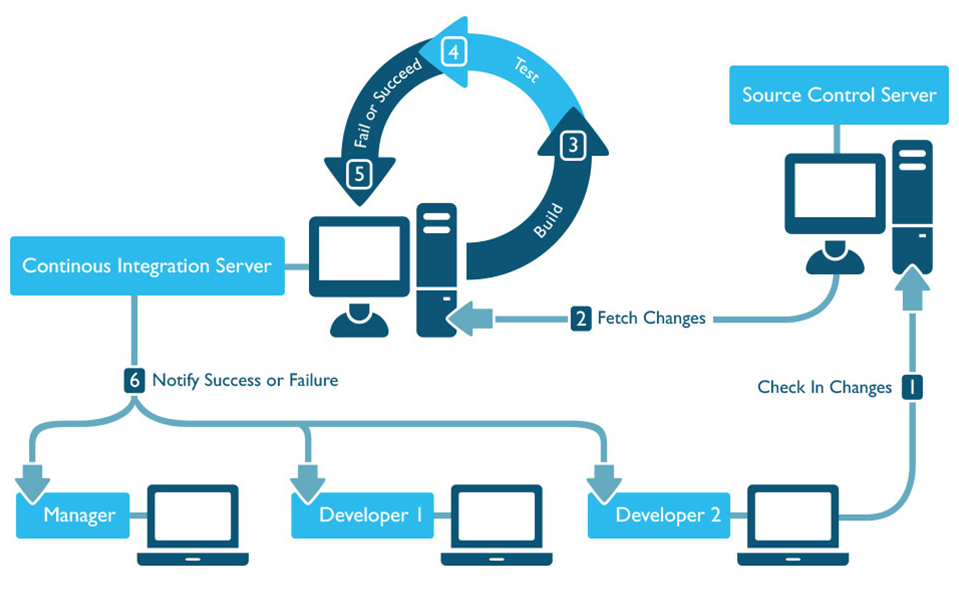
\includegraphics[width=\textwidth]{source/images/ci-flow}
\caption[Technische Umsetzung von \ac{ci}.]{Technische Umsetzung von \ac{ci}, Quelle: \citealt{continuous-improvement}.}
\label{fig:ci-flow}
\end{figure}

Im Wesentlichen beobachtet der \ac{ci}-Server ein \ac{scm} System (2) und führt eine definierte \textit{Build Pipeline} bei jeder Änderung der dazugehörige Codebasis aus (3). So ist es denkbar, dass eine \textit{Build Pipeline} die Codebasis kompiliert, automatisierte Tests ausführt und der Code einer statischen Code Analyse unterzieht (4). Dieser Prozess kann beliebig erweitert und an die Bedürfnisse der einzelnen Teams und deren Projekte angepasst werden. Sollte irgendetwas nicht wie erwartet funktionieren, ein Test fehlschlagen oder gar das Kompilieren der Codebasis misslingen (5), so wird das Team unverzüglich von dem System darüber informiert (6) \citep{jenkins-guide}. 
All das setzt voraus, dass jeder im Team seine \textit{Features} häufig, normalerweise täglich, in das \ac{scm} System integriert (1) \citep{fowler_2006}.

Nach \citet{fowler_2006} ist somit der ganze Sinn einer \ac{ci} schnelles Feedback zu erhalten, um auftretende \textit{Bugs} dadurch frühzeitig zu finden und zu eliminieren, statt diese über lange Zeit in einem \textit{Release} zu kumulieren. Durch die permanente Integration der einzelnen Codebestandteile (\textit{Features}, \textit{Bugfixes}, etc.) wird die Qualität der Software verbessert und Risiken minimiert.

Der \textit{Jenkins} ist ein in \textit{Java} geschriebener \textit{Open Source} \ac{ci}-Server. Die Entwicklung begann im Jahr 2004 durch Kohsuke Kawaguchi, damals unter dem Namen \textit{Hudson} und zählt heute zu den populärsten \ac{ci}-Servern. Dieser wird als Webapplikation bereitgestellt und bietet durch eine große, aktive Community und mehreren hunderten von \textit{Plugins} flexible und diverse Einsatzmöglichkeiten in der permanenten Integration von Softwarekomponenten \citep{jenkins-guide}. \textit{Plugins} bezeichnen Zusatzmodule, die die Basisfunktionalität der eigentlichen Software erweitern. Das \textit{Git Plugin} ermöglicht z.\,B. die Integration eines \textit{Source Code Repositorys} in den \textit{Jenkins}, sodass dieses als Projekt hinzugefügt werden kann und durch den \textit{Jenkins} beobachtet und bei Änderungen analysiert werden kann \citep{git-plugin}.  

\section{Delta-Softwaremetriken}

Nach \citet{augsten_2019} bilden Softwaremetriken bestimmte Eigenschaften von Software als Zahlenwerte ab. Dadurch werden diese vergleichbar und dienen als Maßstab für die Qualität von Software. Beispielsweise bestimmt die \textit{Code Coverage} den prozentualen Anteil des durch automatisierte Tests abgedeckten Quellcodes. Ein Delta bezeichnet im Allgemeinen eine Differenz. 

Eine Delta-Softwaremetrik meint nun die Maßzahl einer bestimmen Softwaremetrik bezogen auf eine Referenz, für die es zwei verschiedene Betrachtungsweisen gibt - die absolute und die relative Referenz.
Bei der absoluten Betrachtung wird als Referenz die gesamte Codebasis des Ziel-\textit{Branches} betrachtet. Das Delta der Metrik gibt also Aufschluss darüber, wie sich die Metrik bezogen auf das Gesamtprojekt durch einen \textit{Pull Request} verändert. 

Ein Beispiel: Auf dem \textit{developer}-\textit{Branch} eines \textit{Repositorys} beträgt die \textit{Code Coverage} 80 \%. Ein Teammitglied entwickelt ein neues \textit{Feature} basierend auf dem \textit{developer}-\textit{Branch} und stellt einen \textit{Pull Request}, damit seine Änderungen in den \textit{developer}-\textit{Branch} integriert werden. Die \textit{Code Coverage} auf dem \textit{feature}-\textit{Branch} beträgt 85 \%. Durch einen erfolgreichen \textit{Merge} wird die \textit{Code Coverage} demnach um 5 \% gesteigert. 

Die relative Betrachtung einer Delta-Metrik bezieht sich dagegen auf den \textit{Pull Request} selbst und gibt an, welche Zeilen des im \textit{Pull Requests} veränderten, gelöschten oder hinzugefügten Quellcodes in der Metrik berücksichtigt sind. 

Ein Beispiel: In einem \textit{Pull Request} wurde der Codebasis eine neue Klasse mit 100 Zeilen hinzugefügt. Für diese Klasse existieren Tests, die den Code automatisiert testen. Diese Tests decken 67 der 100 Zeilen ab. Das bedeutet, dass die Zeilen, die sich in diesem \textit{Pull Request} geändert haben, zu 67 \% durch Tests abgedeckt sind. In der relativen Delta-Betrachtung, besitzt dieser \textit{Pull Request} demnach eine \textit{Code Coverage} von 67 \%. Diese Delta-Betrachtung reduziert die Kennzahl der jeweiligen Softwaremetrik also auf die im \textit{Pull Request} veränderten Codezeilen, anstatt das Gesamtprojekt zu beurteilen. 

Häufig sind es diese Delta-Betrachtungen, die bei einem \textit{Pull Request} relevant sind und für die \textit{Reviewer} von Interesse sind, um die Qualität eines \textit{Pull Requests} und der darin enthaltenen Weiterentwicklung beurteilen zu können. 


